\chapter{Kreisbewegung}
Bei einer Kreisbewegung verläuft die Bahnkurve kreisförmig,
d.h. die bewegte Masse hat eine zusammengesetzte Beschleunigung.
Diese setzt sich aus einem radialen und tangentialen Anteil 
zusammen. Da eine beschleunigte Masse eine Kraft ausübt, wird 
bei einer Kreisbewegung auch von Radial- bzw. Zentripetalkraft
(eine nach innen, zum Zentrum gerichtete Kraft) und der 
Tangentialkraft (eine tangential anliegende Kraft) gesprochen.

\newpage
\section{Gleichförmige Kreisbewegung}
Bei einer gleichförmigen Kreisbewegung ist die Bahngeschwindigkeit
konstant und hat einen konstanten Abstand (Radius) zum Mittelpunkt.

\begin{figure}[h!]
	\centering
	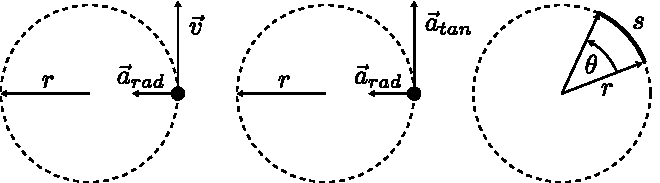
\includegraphics[scale=0.8]{../fig/kreisbewegung.pdf}
	\caption{Gleichförmige Kreisbewegung}
	\label{fig:kreisbewegung}
\end{figure}

\noindent
Die radial wirkende Kraft welche auch als Zentripetalkraft 
bezeichnet wird, kann auf verschiedene Weise berechnet werden.
\[ \boxed{\vec{F}_{rad} = \vec{F}_{ZP} 
	= m \cdot \vec{a}_{rad}
	= m \cdot \frac{\vec{v}^2}{r} 
	= m \cdot \omega^2 \cdot r 
	= m \cdot \frac{4 \cdot \pi^2 \cdot r}{T^2} } \]
Die Beziehungen zwischen den Bahngrössen lassen sich dabei 
grundsätzlich mit vier Gleichungen beschreiben:
\[ \boxed{ \begin{array}{l r c l}
	\text{Bogenlänge $s$} & 
		s &=& r \cdot \theta \\
	& & & \\
	\text{Geschwindigkeit tangential $\vec{v}$} &
		\vec{v} &=& r \cdot \omega
		= r \cdot \frac{d\theta}{dt} \\
	& & & \\
	\text{Beschleunigung tangential $\vec{a}_{tan}$} &
		\vec{a}_{tan} &=& r \cdot \alpha 
		= r \cdot \frac{d^2\theta}{dt} \\
	& & & \\
	\text{Beschleunigung radial $\vec{a}_{rad}$} &
		\vec{a}_{rad} &=& \frac{v^2}{r} = \omega^2 \cdot r
\end{array} }\]

\noindent
Wichtig ist dabei stets den Zusammenhang zwischen den verschiedenen 
Beschleunigungen eines rotierenden Körpers zu beachten.
\[ \boxed{\begin{array}{r c l}
	\vec{a}_{rad} 
		&=& \displaystyle \frac{\vec{v}^2}{r} 
		= \displaystyle \omega^2 \cdot r
		= \displaystyle \left(\frac{d\theta}{dt}\right)^2 \cdot r
		= \displaystyle \dot{\theta}^2 \cdot r \\
	& & \\
	\vec{a}_{tan} 
		&=& \displaystyle \alpha \cdot r
		= \displaystyle \left(\frac{d^2\theta}{dt^2}\right) \cdot r
		= \displaystyle \ddot{\theta} \cdot r \\
	& & \\
	\vec{a}_{res} 
		&=& \sqrt{\vec{a}_{rad}^2 + \vec{a}_{tan}^2} 
\end{array} }\]

\section{Winkelbetrachtung}\label{sec:winkelbetrachtung}
Bei Kreisbewegungen ist es von Vorteil, wenn die Bewegung nicht als
Weg pro Zeit ($\frac{m}{s}$) sondern als Winkel pro Zeit 
($\frac{rad}{s}$) betrachtet wird. Eine Kreisbewegung kann somit 
unabhängig vom Radius beschrieben werden. In diesem Fall spricht
man dann von der Winkelgeschwindigkeit $\omega$ und 
Winkelbeschleunigung $\alpha$. Mit dieser Betrachtungsweise kann
eine Kreisbewegung analog zur Translation beschrieben werden, denn
auch hier gilt der Zusammenhang von Weg, Geschwindigkeit und 
Beschleunigung wie in der Translation.

\[ \boxed{ \begin{array}{l l}
	\text{Rotation} \qquad &
		\theta
		\xrightarrow{\frac{d}{dt}} \omega 
		\xrightarrow{\frac{d}{dt}} \alpha \\
	& \\
	\text{Translation} \qquad &
		s
		\xrightarrow{\frac{d}{dt}} \vec{v} 
		\xrightarrow{\frac{d}{dt}} \vec{a}
\end{array} }\]

\noindent
Die einzelnen Grössen $\omega$ und $\alpha$ können mit den folgenden 
Formeln beschrieben werden.
\[ \boxed{\begin{array}{l r c l}
	\text{Winkelgeschwindigkeit} &
		\omega &=& \omega_0 + \alpha \cdot t 
			= \displaystyle \frac{d\theta}{dt} 
			= \displaystyle \dot{\theta} \\
	& & \\
	\text{Winkelbeschleunigung} &
		\alpha &=& \displaystyle \frac{d^2\theta}{dt^2} = \ddot{\theta}
\end{array} }\]

\section{Drehmoment}
Wirkt eine Kraft nicht auf die Drehachse eines Körpers, so ergibt
sich aus dem Vektorprodukt von Versatz und Kraft das sogenannte
Drehmoment.

\begin{figure}[h!]
	\centering
	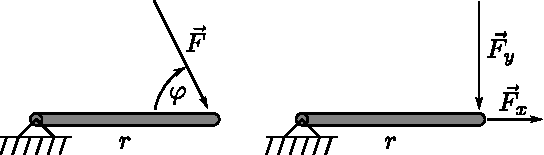
\includegraphics[scale=0.8]{../fig/drehmoment.pdf}
	\caption{Drehmoment komponentenweise betrachtet.}
	\label{fig:drehmoment}
\end{figure}

\noindent
Die Grafik \ref{fig:drehmoment} zeigt ein einfaches Beispiel der
komponentenweisen Betrachtung von Kräften. Im Beispiel bewirkt lediglich
die Komponente $\vec{F}_y$ ein Drehmoment, denn $\vec{F}_x$ wirkt auf
die Drehachse und erzeugt somit kein Drehmoment.

\[ \boxed{\begin{array}{l c l} 
	\vec{M} &=& \vec{r} \times \vec{F}
			\qquad \qquad
		\vec{M} = \vec{r} \cdot \vec{F}
			\quad \text{falls } \quad \vec{r} \bot \vec{F} \\
	& & \\ 
	\vec{M} 
		&=& r \cdot \vec{F}_\bot 
		= r \cdot \vec{F} \cdot sin(\varphi) \\
\end{array} }\]

\noindent
Wirken mehrere Kräfte auf verschiedene Punkte eines Körpers, so können
die einzelnen Drehmomente zum Gesamtdrehmoment summiert werden.
\[ \boxed{
	\vec{M} = \sum \left(\vec{r}_i \times \vec{F}_i\right)
	= \left(\vec{r}_1 \times \vec{F}_1 \right)
		+ \left( \vec{r}_2 \times \vec{F}_2 \right)
		+ \dots 
		+ \left( \vec{r}_n \times \vec{F}_n \right)
} \]
Analog zur linearen Bewegung kann auch bei der Betrachtung von Drehmomenten
das zweite Newton'sche Axiom angewandt werden, denn ein resultierendes
Drehmoment bewirkt eine Änderung der Winkelgeschwindigkeit $\alpha$.

Betrachtet man das Drehmoment von rotierenden Körpern, so können die
Zusammenhänge von Masseverteilung (siehe Kapitel 
\ref{sec:traegheitsmoment}) und Drehbewegung genutzt werden zur
Formulierung des Drehmomentes. Ein Drehmoment kann so beschrieben werden
als das Produkt aus dem Trägheitsmoment $I$ und der Winkelbeschleunigung
$\alpha$, als Differential des Drehimpulses $L$ oder als Verhältnis von 
Leistung $P$ und Drehzahl $n$ (Umdrehungen pro Sekunde).
\[ \boxed{\begin{array}{r c l}
	\vec{M}
		&=& \displaystyle \vec{r} \times \vec{F}
			\qquad \qquad \rightarrow \vec{r} \bot \vec{F} 
			\Rightarrow \vec{M} = \vec{r} \cdot \vec{F} \\
	& & \\
	\vec{M} 
		&=& \displaystyle I \cdot \alpha \\
	& & \\
	\vec{M} 
		&=& \displaystyle \frac{d\vec{L}}{dt} \\
	& & \\
	\vec{M} 
		&=& \displaystyle \frac{P}{2 \cdot \pi \cdot n}
\end{array} }\]

\section{Drehimpuls}
Der Drehimpuls beschreibt den \textit{Drall} eines rotierenden Körpers
und ist eine vektorielle Grösse, d.h. der Drehimpuls hat sowohl einen
skalaren Betrag (Norm des Vektors) als auch eine Richtung. Dies kommt
daher, dass der Drehimpuls das Vektor- oder Kreuzprodukt aus Radius und
Impuls ist (das ergibt einen Vektor der normal auf der Ebene von 
$\vec{r},\vec{p}$ steht).
\[ \boxed{
	\vec{L}
		= \vec{r} \times \vec{p}
		= \vec{r} \times(m \cdot \vec{v})
}\]

\noindent
Wird zur Ermittlung des Drehimpulses eine gemeinsame Referenz im Raum
gewählt, so kann direkt das Trägheitsmoment eines Körpers verwendet
werden (die Drehachse muss dabei fest im Raum liegen).
\[ \boxed{
	\vec{L} = I \cdot \vec{\omega} 
	\quad \leftrightarrow \quad
	\vec{M} = I \cdot \vec{\alpha}
} \]

\noindent
Der Drehimpuls ist wie der Impuls in der linearen Bewegung eine 
Erhaltungsgrösse. Analog zu den Kräften in der Rotation 
sind es die Drehmomente in der Rotation. 
\[ \boxed{
	\sum \vec{M}_{extern} = 0 
	\quad \Rightarrow \quad 
	\vec{L} = konstant
} \]

\section{Trägheitsmoment}\label{sec:traegheitsmoment}
Das Trägheitsmoment beschreibt die Massenverteilung eines Körpers
bezogen auf eine Drehachse. Dieses muss bei jeder Form von Rotation
berücksichtigt werden und ist grundsätzlich unabhängig von der 
Bewegung, nicht aber von der Drehachse.

Das Trägheitsmoment wird beschrieben durch die Summe der 
Produkte aus den Massepunkten und deren Abstand im Quadrat zur 
Drehachse des Körpers.
\[ \boxed{
	I = \left(m_1 \cdot r_1^2 \right)
		+ \left( m_2 \cdot r_2^2 \right)
		+ \dots 
		+ \left( m_n \cdot r_n^2 \right)
		= \sum m_i \cdot r_i^2
		= \int r^2 \cdot dm
} \]

\noindent
Trägheitsmomente verschiedener Körper können zu einem Trägheitsmoment
summiert werden, wenn diese auf der gleichen Drehachse rotieren.
\[ \boxed{
	I_{Total} = I_1 + I_2 + \dots + I_n
} \]

\newpage
\subsection{Trägheitsmomente regelmässiger Körper}

\begin{table}[h!]
\centering
\begin{tabular}{m{2cm} c m{0.4\textwidth}}
Körper	& Achse	& $I$ \\
\hline
& & \\
Kreisring, dünn &
	\begin{minipage}{0.3\textwidth}
	\centering
	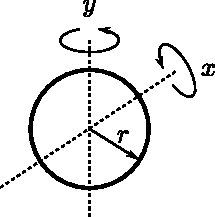
\includegraphics[scale=\traegscale]{../fig/traeg-kreisring-duenn.pdf}
	\end{minipage} &
		\begin{itemize}
		\item[x:] $m \cdot r^2$
		\item[y:] $\frac{m}{2} \cdot r^2$
		\end{itemize} \\
Kreisring &
	\begin{minipage}{0.3\textwidth}
	\centering
	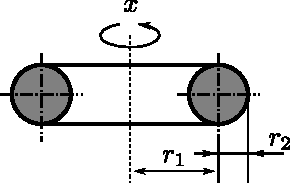
\includegraphics[scale=\traegscale]{../fig/traeg-kreisring.pdf}
	\end{minipage} &
		\begin{itemize}
			\item[x:] $m \cdot \left({r_1}^2 + \frac{3}{4}
				\cdot {r_2}^2\right)$
		\end{itemize} \\
Kreisbogen &
	\begin{minipage}{0.3\textwidth}
	\centering
	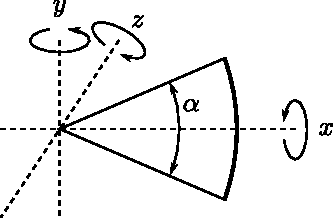
\includegraphics[scale=\traegscale]{../fig/traeg-kreisbogen.pdf}
	\end{minipage} &
		\begin{itemize}
		\item[x:] $\frac{m}{2}r^2 
			\left(1-\frac{sin(\alpha)}{\alpha} \right)$
		\item[y:]  $\frac{m}{2}r^2 
			\left(1+\frac{sin(\alpha)}{\alpha} \right)$
		\item[z:] $mr^2$
		\end{itemize} \\
Kreissektor &
	\begin{minipage}{0.3\textwidth}
	\centering
	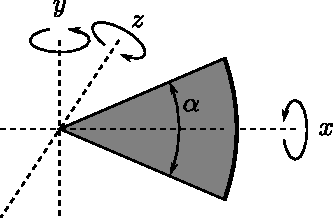
\includegraphics[scale=\traegscale]{../fig/traeg-kreissektor.pdf}
	\end{minipage} &
		\begin{itemize}
		\item[x:] $\frac{m}{4} r^2  
			\left(1-\frac{sin(\alpha)}{\alpha} \right)$
		\item[y:]  $\frac{m}{4} r^2 
			\left(1+\frac{sin(\alpha)}{\alpha} \right)$
		\item[z] $\frac{m}{2} r^2$	
		\end{itemize} \\
Kreisscheibe, dünn &
	\begin{minipage}{0.3\textwidth}
	\centering
	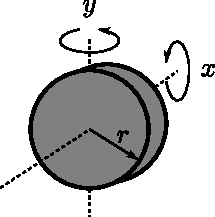
\includegraphics[scale=\traegscale]{../fig/traeg-kreisscheibe-duenn.pdf}
	\end{minipage} &
		\begin{itemize}
		\item[x:] $\frac{m}{2} r^2$
		\item[y:] $\frac{m}{4} r^2$
		\end{itemize} \\
Kugel, solid & \multirow{2}{*}{
	\begin{minipage}{0.3\textwidth}
	\centering
	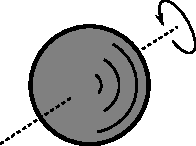
\includegraphics[scale=\traegscale]{../fig/traeg-kugel.pdf}
	\end{minipage}}
		&
		\begin{itemize}
			\item[x:] $\frac{2}{5} mr^2$
		\end{itemize} \\
Kugel, dünnwandig & &
		\begin{itemize}
			\item[x:] $\frac{2}{3} mr^2$
		\end{itemize}
\end{tabular}
\end{table}

\newpage
\begin{table}[h!]
\centering
\begin{tabular}{m{2cm} c m{0.4\textwidth}}
Körper	& Achse	& $I$ \\
\hline
& & \\
Stab &
	\begin{minipage}{0.3\textwidth}
	\centering
	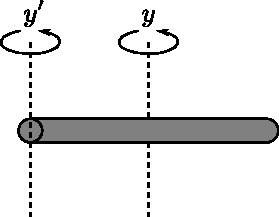
\includegraphics[scale=\traegscale]{../fig/traeg-stab.pdf}
	\end{minipage} &
		\begin{itemize}
		\item[y:] $\frac{m}{12} l^2$
		\item[y':] $\frac{1}{3} m l^2$
		\end{itemize} \\
& & \\
Vollzylinder &
	\begin{minipage}{0.3\textwidth}
	\centering
	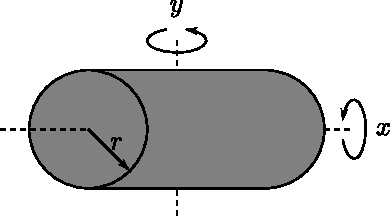
\includegraphics[scale=\traegscale]{../fig/traeg-vollzylinder.pdf}
	\end{minipage} &
		\begin{itemize}
		\item[x:] $\frac{m}{2} r^2$
		\item[y:] $\frac{m}{12} \left( 3r^2 + h^2 \right)$
		\end{itemize} \\
& & \\
Hohlzylinder, dünnwandig &
	\begin{minipage}{0.3\textwidth}
	\centering
	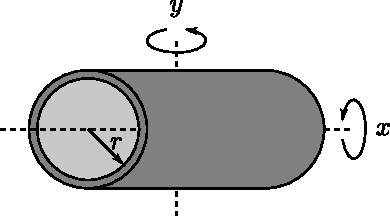
\includegraphics[scale=\traegscale]{../fig/traeg-hohlzylinder-duenn.pdf}
	\end{minipage} &
		\begin{itemize}
		\item[x:] $mr^2$
		\item[y:] $\frac{m}{4} (2r^2 + \frac{h^2}{3})$
		\end{itemize} \\
& & \\
Hohlzylinder &
	\begin{minipage}{0.3\textwidth}
	\centering
	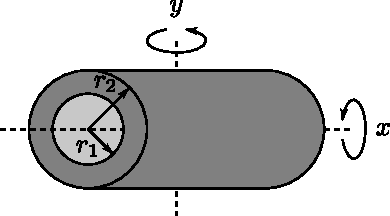
\includegraphics[scale=\traegscale]{../fig/traeg-hohlzylinder.pdf}
	\end{minipage} &
		\begin{itemize}
		\item[x:] $\frac{m}{2} \left({r_1}^2 + {r_2}^2 \right)$
		\item[y:] $\frac{m}{4} \left({r_1}^2 + {r_2}^2 
			+ \frac{h^2}{3} \right)$
		\end{itemize}\\
Quader &
	\begin{minipage}{0.3\textwidth}
	\centering
	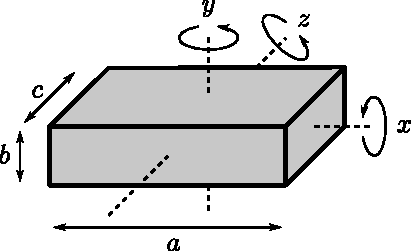
\includegraphics[scale=\traegscale]{../fig/traeg-quader.pdf}
	\end{minipage} &
		\begin{itemize}
		\item[x:] $\frac{m}{12} \left(b^2 + c^2\right)$
		\item[y:] $\frac{m}{12} \left(a^2 + c^2\right)$
		\item[z:] $\frac{m}{12} \left(a^2 + b^2\right)$
		\end{itemize} \\
Platte, dünn &
	\begin{minipage}{0.3\textwidth}
	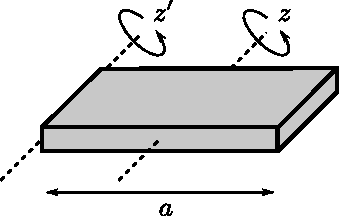
\includegraphics[scale=\traegscale]{../fig/traeg-platte.pdf}
	\end{minipage} &
		\begin{itemize}
		\item[z:] $\frac{m}{12} a^2$
		\item[z':] $\frac{1}{3} ma^2$
		\end{itemize} \\
\end{tabular}
\end{table}

\newpage
\section{Achsenbezogene Trägheitsmomente}
Bei der Betrachtung von Trägheitsmomenten zu einer bestimmten Achse gibt 
es zwei grundlegende Sätze die zur Berechnung verwendet werden können:

\begin{itemize}
	\item Satz von Steiner (Satz über parallele Achsen)
	\item Satz über senkrechte Achsen
\end{itemize}

\subsection{Parallele Achsen (Satz von Steiner)}
\begin{figure}[h!]
	\centering
	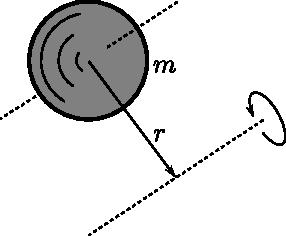
\includegraphics[scale=0.7]{../fig/steiner.pdf}
	\caption{Kugel mit um $r$ versetzter Drehachse.}
	\label{fig:steiner}
\end{figure}

\noindent
Der Steiner'sche Satz (auch Parallelachsen-Theorem) wird angewandt um
das Trägheitsmoment eines Körpers zu berechnen, wenn dessen Drehachse nicht
durch den Schwerpunkt des Körpers geht. Der Satz besagt, dass dies für 
jeden Körper gleich berechnet werden kann wenn
\begin{itemize}
	\item das Trägheitsmoment für die Drehachse durch den Schwerpunkt
		bekannt ist
	\item die versetzte Drehachse parallel zur Drehachse durch den
		Schwerpunkt geht
\end{itemize}
Sind diese Bedingungen erfüllt kann das Trägheitsmoment nach Steiner
berechnet werden.
\[ \boxed{ I_{Parallel} = I_{Schwerpunkt} + m \cdot r^2 } \]
Aus der obigen Formel geht hervor, dass das Trägheitsmoment bei versetzter
Drehache stets grösser ist, als mit einer Drehachse durch den Schwerpunkt
(da $m,r>0$ sein muss).

\subsection{Senkrechte Achsen}
Flache Körper, also Körper deren Höhe vernachlässigt werden kann, können
mittels des Satzes über senkrechte Achsen betrachtet werden.

\begin{figure}[h!]
	\centering
	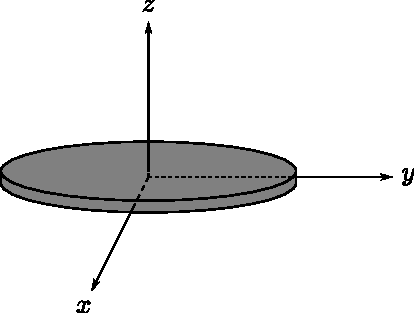
\includegraphics[scale=0.8]{../fig/steiner2.pdf}
	\caption{Flache Scheibe mit der Ebene $(x,y)$.}
	\label{fig:steiner2}
\end{figure}

\noindent
Der Satz besagt am Beispiel der Grafik \ref{fig:steiner2}, 
dass das Trägheitsmoment senkrecht zur Ebene $(x,y)$ des 
Körpers die Summe der zur Achse $z$ senkrecht stehenden Trägheitsmomente 
ist. Dieser Satz gilt nur wenn
\begin{itemize}
	\item die Trägheitsmomente für $x,y,z$ durch den Schwerpunkt des 
		Körpers gehen
	\item die Trägheitsmomente für $x$ und $y$ senkrecht zueinander 
		sind, also $x \bot y$ gilt
	\item die Masse gleichmässig (also homogen) verteilt ist
\end{itemize}
Sind diese Bedingungen erfüllt, kann das Trägheitsmoment nach dem Satz
über senkrechte Achsen berechnet werden.
\[ \boxed{I_z = I_x + I_y} \]
Dieser Satz ist besonders dann geeignet, wenn ein Körper der Form einer
Scheibe betrachtet wird (siehe Bild \ref{fig:steiner2}). 
Denn wenn der Körper einen perfekten Kreis abbildet mit konstantem 
Radius $r$, dann muss $I_x = I_y$ gelten und somit auch 
$\frac{1}{2} I_z = I_x = I_y$.

\newpage
\section{Perfektes Rollen}\label{sec:non-slip}
Bei der Betrachtung von Rotationen gibt es einen Spezialfall welcher
als perfektes Rollen bezeichnet wird (engl. \textit{non slip condition}).
Hierbei meint man eine Rotation eines Körper über einer Auflage (z.B. 
Untergrund, Seil etc.) wobei stets die Haftreibung herrscht. 
Ein einfaches Beispiel aus dem Alltag ist das Rad, welches ideal bzw. 
perfekt rollt ohne zu rutschen.

\begin{figure}[h!]
	\centering
	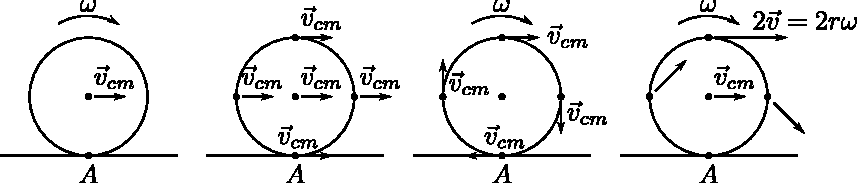
\includegraphics[width=0.95\textwidth]{../fig/non-slip.pdf}
	\caption{Non-Slip Condition.}
	\label{fig:non-slip}
\end{figure}

\noindent
Die Grafik \ref{fig:non-slip} illustriert am Beispiel des Rades wie die 
Translation und Rotation kombiniert wird (von links nach rechts).
\begin{itemize}
	\item{Bild 1:} Das Rad bewegt sich mit $\vec{v}_{cm}$ vorwärts und
		dreht sich mit $\omega$ und die Drehachse im Mittelpukt.
	\item{Bild 2:} Translation des Rades mit $\vec{v}_{cm}$.
	\item{Bild 3:} Rotation des Rades mit $\omega$ um die Drehachse.
		Jeder Massepunkt bewegt sich dabei mit $\vec{v}_{cm}$
		tangential zur Drehachse.
	\item{Bild 4:} Rotation und Translation kombiniert sich bei
		Drehachse im Auflagepunkt $A$ (dort ist $\vec{v}=0$).
\end{itemize}
Die Bewegung eines rollenden Rades setzt sich also aus zwei Bewegungen
zusammen; einer Translation und einer Rotation. Gilt dabei die sog. 
non slip condition, so können diese Bewegungen kombiniert betrachtet 
werden, indem die Drehachse zum Auflagepunkt hin verschoben wird. 
\[ \boxed{\begin{array}{c c c c c c c}
		& & x_{cm} 
		&=& r \cdot \theta 
		& & \\
	\vec{v}_{cm} 
		&=& \dot{x}_{cm} 
		&=& r \cdot \dot{\theta }
		&=& r \cdot \omega \\
	\vec{a}_{cm} 
		&=& \ddot{x}_{cm}
		&=& r \cdot \ddot{\theta}
		&=& r \cdot \alpha
\end{array}}\]

\subsection{Reibungskraft und Trägheit}
Bei der Betrachtung von Rotationen welche die sogenannte 
\textit{non-slip condition} erfüllen, also perfekt rollen, können die 
zum Rollen nötige Reibungskraft $\vec{F}_R$ und die Scheinkraft der 
translativen Trägheit $\vec{F}_T$ leicht bestimmt werden.

\begin{figure}[h!]
	\centering
	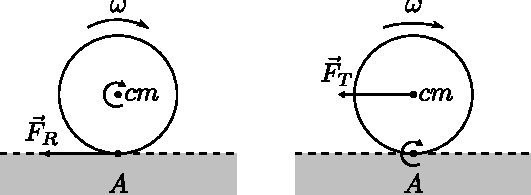
\includegraphics[scale=0.8]{../fig/non-slip-kraft.pdf}
	\caption{Reibungskraft $\vec{F}_R$ die im Auflagepunkt 
		wirkt für Drehachse bei $cm$ und 
		Trägheit die auf $cm$ wirkt bei Drehachse bei A}
	\label{fig:non-slip-kraft}
\end{figure}

\noindent
Hierzu muss jeweils die richtige Drehachse gewählt werden (siehe
Grafik \ref{fig:non-slip-kraft}) und je nach Situation der Satz von
Steiner angewandt werden. Hat der betrachtete Körper keine Translation
so wird die Trägheit mit $I_A=0$ berechnet (typisch bei 
massebehafteten Rollen etc.)!

\[ \boxed{\begin{array}{l c l}
	\text{Reibung } \vec{F}_R 
		& \xrightarrow{rot_{cm}}
		& I = I_{cm} \\
	 & & \\
	\text{Trägheit } \vec{F}_T 
		& \xrightarrow{rot_A}
		& I = I_{cm} + I_A \qquad,I_A = m \cdot r^2
\end{array}}\]

\[ \boxed{\begin{array}{c c l}
	\vec{F}_R \cdot r 
		& =
		& \vec{M}_{cm} = I_{cm} \cdot \alpha 
		\qquad \xrightarrow{non-slip} 
			\displaystyle
			\alpha = \frac{\vec{a}_{cm}}{r} \\
%	& & \\
%	 	& \Rightarrow 
%		& \vec{F}_R \cdot r 
%			= \displaystyle 
%				(C \cdot m \cdot r^2) 
%				\cdot \frac{\vec{a}_{cm}}{r}
%			= \displaystyle 
%				C \cdot m \cdot r 
%				\cdot \vec{a}_{cm} \\
	& & \\
		& \Rightarrow 
		& \vec{F}_R = C \cdot m \cdot \vec{a}_{cm} \\
	& & \\
	& & \\
	\vec{F}_T \cdot r 
		& = 
		& \vec{M}_{A} = (I_{cm} + I_P) \cdot \alpha
		\qquad \xrightarrow{non-slip}
			\displaystyle
			\alpha = \frac{\vec{a}_{cm}}{r} \\
%	& & \\
%		& \Rightarrow
%		& \vec{F}_T \cdot r = \displaystyle
%			(I_{cm}+I_A) \cdot \frac{\vec{a}_{cm}}{r} \\
%	& & \\
%		& =
%		& \vec{F}_T \cdot r = \displaystyle 
%			(C \cdot m \cdot r^2 + m \cdot r^2) \cdot 
%			\frac{\vec{a}_{cm}}{r} \\
	& & \\
		& \Rightarrow 
		& \vec{F}_T = (C + 1) \cdot m \cdot \vec{a}_{cm}
\end{array} } \]

\section{Rotationsenergie}
Die Rotationsenergie ist im Grunde genommen die kinetische Enerige
eines starren Körpers der um eine feste Achse rotiert.
\[ \boxed{\begin{array}{r c l}
E_{kin} 
		&=& \frac{1}{2} \cdot m \cdot \vec{v}^2 \\
	& & \\
	\Rightarrow E_{rot} 
		&=& \frac{1}{2} \cdot m_1 \cdot \vec{v}_1^2
			+ \frac{1}{2} \cdot m_2 \cdot \vec{v}_2^2
			+ \dots 
			+ \frac{1}{2} \cdot m_n \cdot \vec{v}_n^2 \\
	& & \\
		&=& \frac{1}{2} \cdot \left(m_1 \cdot r_1^2
			+ m_2 \cdot r_2^2 
			+ \dots
			+ m_n \cdot r_n^2\right) \cdot \omega^2 \\
	& &\\
		&=& \frac{1}{2} \cdot I \cdot \omega^2 
\end{array} } \]
Bei der Berechnung der Bewegungsenergie aus Translation und 
Rotation muss auf die Lage der Drehachse geachtet werden. Insbesondere 
gilt beim perfekten Rollen (siehe Kapitel \ref{sec:non-slip}) der 
folgende Zusammenhang.
\[ \boxed{\begin{array}{r c l}
	E_B 
		&=& E_{kin_{Translation}} + E_{kin_{Rotation}} \\
	& \\
	E_B 
		&=& \frac{1}{2} \cdot m_T \cdot {\vec{v}_{cm}}^2 
			+ \frac{1}{2} \cdot I \cdot \omega^2 
\end{array}}\]
Die Masse $m_T$ ist die Summe aller translativ bewegter Massen. D.h. 
wendet man die non-slip condition an und wählt die Drehachse an einem 
versetzten Punkt (z.B. Auflagepunkt eines Rades), so müssen die nun
rotierenden Massen von $m_T$ abgezogen werden, denn diese sind dann in
der Rotation enthalten.
\newpage
\section{Rotation vs. Translation}
Wie im Kapitel \ref{sec:winkelbetrachtung} beschrieben, kann die 
Rotation analog zur Translation betrachtet werden.

\[ \boxed{\begin{array}{l l}
\textbf{Rotation} & \textbf{Translation} \\
& \\
\text{Winkelbeschleunigung $\left[\frac{rad}{s^2}\right]$}
	& \text{Beschleunigung $\left[\frac{m}{s^2}\right]$} \\
		\qquad \alpha = \frac{d^2\theta}{dt^2} = \ddot{\theta}
			& \qquad \vec{a} = \frac{d^2s}{dt^2} \\
& \\
\text{Winkelgeschwindigkeit $\left[\frac{rad}{s}\right]$} 
	& \text{Geschwindigkeit $\left[\frac{m}{s}\right]$} \\
		\qquad \omega = \frac{d\theta}{dt} = \dot{\theta} 
			& \qquad \vec{v} = \frac{ds}{dt} \\
& \\
\text{Winkel $\left[rad\right]$} 
	& \text{Weg $\left[ m \right]$} \\
		\qquad \theta = \omega_0 \cdot t + \frac{1}{2} \cdot \alpha \cdot t^2
			& \qquad s = \vec{v}_0 \cdot t + \frac{1}{2} \cdot \vec{a} \cdot t^2 \\
		& \\
		\qquad \theta = \frac{1}{2} \cdot (\omega + \omega_0) \cdot t
			& \qquad s = \frac{1}{2} \cdot (\vec{v} + \vec{v}_0) \cdot t \\
& \\
\text{Trägheitsmoment $\left[kg \cdot m^2\right]$} 
	& \text{Masse $\left[kg\right]$} \\
		\qquad I = \sum r_i^2 \cdot m_i = \int r^2 \cdot dm
			& \qquad m \\
& \\
\text{Drehmoment $\left[N \cdot m\right]$}
	& \text{Kraft $\left[N\right]$} \\
		\qquad M = I \cdot \alpha
			& \qquad \vec{F} = m \cdot \vec{a} \\
& \\
\text{Drehimpuls $\left[\frac{kg \cdot m^2}{s}\right]$} 
	& \text{Impuls $\left[N \cdot s\right]$} \\
		\qquad L = I \cdot \omega 
			= r \times \vec{p}
			& \qquad \vec{p} = m \cdot \vec{v} \\
& \\
\text{Rotationsenergie $\left[J\right]$} 
	& \text{Kinetische Energie $\left[J\right]$} \\
		\qquad E_{Rot} = \frac{1}{2} \cdot I \cdot \omega^2
			& \qquad E_{Kin} = \frac{1}{2} \cdot m \cdot \vec{v}^2 \\
& \\
\text{Leistung $\left[W\right]$}
	& \text{Leistung $\left[W\right]$} \\
		\qquad P = \frac{dE}{dt} = M \cdot \omega 
			& \qquad P = \vec{F} \cdot \vec{v}
\end{array} } \]


